% !TEX program = pdflatex
% !TEX root = Manual.tex
\documentclass[12pt,a4paper]{article}
\usepackage[utf8]{inputenc}
\usepackage{babel}
\usepackage{geometry}
\usepackage{graphicx}
\usepackage{fancyhdr}
\usepackage{float}
\usepackage{array}
\usepackage{booktabs}
\usepackage{tabularx}
\usepackage{hyperref}

\geometry{margin=2.5cm}
\setlength{\headheight}{14.5pt}

\pagestyle{fancy}
\fancyhf{}
\lhead{Paradigmas de Programacion}
\rhead{Manual de Usuario 2048}
\cfoot{\thepage}

\title{
	\textbf{Instituto Tecnologico de Costa Rica} \\
	\large Escuela de Ingenieria en Computacion \\
	\large Paradigmas de Programacion (CE 2048) \\
	\vspace{0.5cm}
	\Large \textbf{Manual de Usuario: Juego 2048 en Racket}
}

\author{Jeremy Serracin Oporta - 2022164175 \\
Sebastian Bolanos Zamora - 2024099520 \\
Andres Madrigal Vega - 2021572460}

\date{9 de Abril de 2026}

\begin{document}

\maketitle
\thispagestyle{empty}

\tableofcontents
\newpage

\section{Introduccion}

Este manual describe como ejecutar y utilizar el juego 2048 distribuido como ejecutable.
Su objetivo es guiar al usuario final paso a paso para iniciar una partida, entender
la interfaz, usar los controles y resolver problemas comunes de ejecucion.

\section{Objetivo del juego}

El objetivo de 2048 es combinar fichas con el mismo valor hasta alcanzar la ficha \textbf{2048}.
En cada turno, todas las fichas se desplazan en la direccion elegida por el jugador, y despues
de cada movimiento valido aparece una nueva ficha en una casilla vacia.

\section{Requisitos}

\subsection{Software requerido}
\begin{itemize}
	\item Sistema operativo compatible con el ejecutable (Linux, Windows o macOS).
\end{itemize}

\subsection{Archivos necesarios}
Para ejecutar el juego, debe estar disponible el archivo ejecutable correspondiente al sistema operativo.
\begin{itemize}
	\item Linux/macOS: \texttt{2048} (o el nombre entregado para el binario).
	\item Windows: \texttt{2048.exe} (o el nombre entregado para el binario).
\end{itemize}

\section{Ejecucion del juego}

\subsection{Opcion A: ejecucion directa (doble clic)}
\begin{enumerate}
	\item Ubicar el ejecutable del juego en el explorador de archivos.
	\item Ejecutarlo con doble clic (o con la opcion \textit{Abrir/Ejecutar}).
	\item Responder en consola las preguntas iniciales del programa.
\end{enumerate}

\begin{figure}[H]
	\centering
	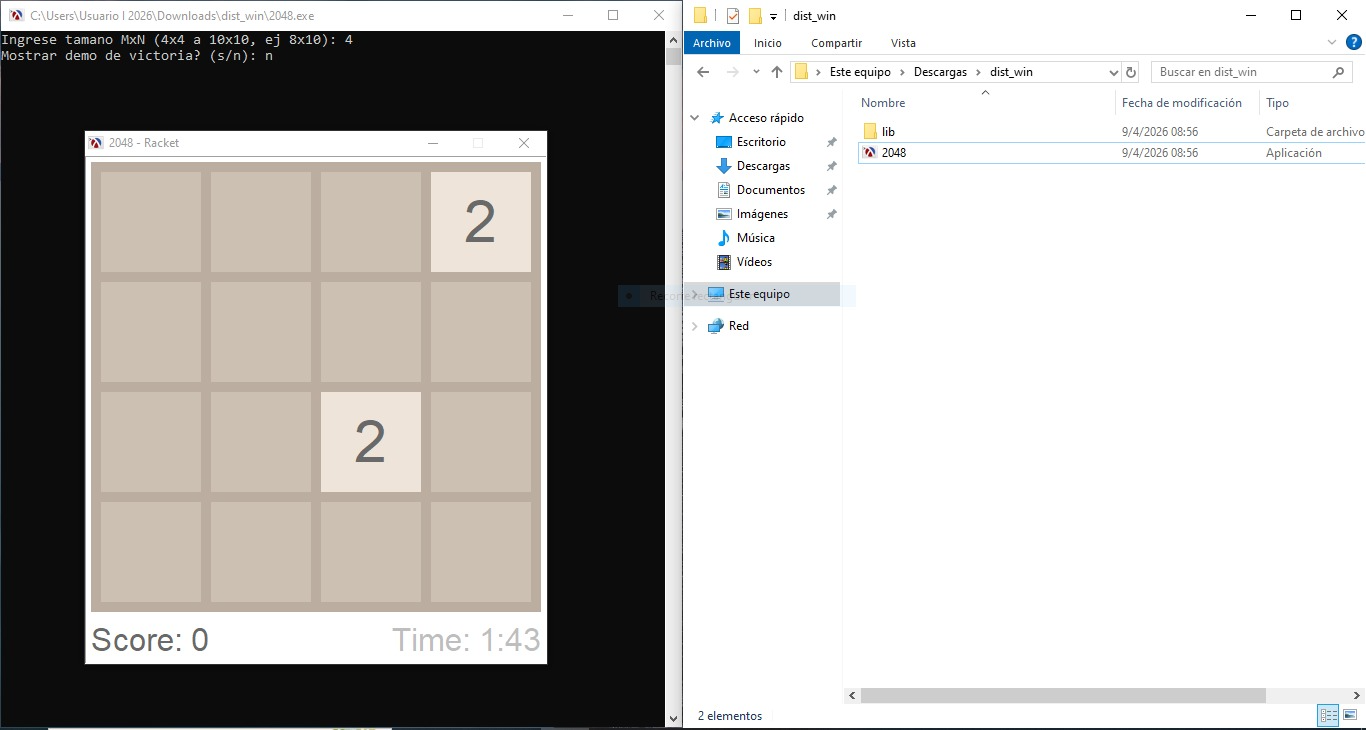
\includegraphics[width=0.85\textwidth]{imagenes/exe-run.png}
	\caption{Ejecucion del juego desde ejecutable.}
	\label{fig:exe-run}
\end{figure}

\subsection{Opcion B: desde terminal (ejecutable)}
\begin{enumerate}
	\item Abrir terminal.
	\item Ubicarse en la carpeta del proyecto.
	\item En Linux/macOS, si aplica, dar permisos: \texttt{chmod +x 2048}
	\item Ejecutar el binario:
	\begin{itemize}
		\item Linux/macOS: \texttt{./2048}
		\item Windows: \texttt{2048.exe}
	\end{itemize}
\end{enumerate}

\begin{figure}[H]
	\centering
	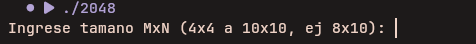
\includegraphics[width=0.85\textwidth]{imagenes/terminal-run.png}
	\caption{Ejecucion del ejecutable desde terminal.}
	\label{fig:terminal-run}
\end{figure}

\section{Flujo inicial de uso}

Al iniciar el programa, se solicitan dos entradas:

\subsection{Tamano del tablero}
El programa pide un tamano en formato \texttt{MxN} con valores entre 4 y 10.

\textbf{Entradas validas:}
\begin{itemize}
	\item \texttt{4x4}
	\item \texttt{8x10}
	\item \texttt{6} (equivale a \texttt{6x6})
\end{itemize}

\textbf{Entradas invalidas:}
\begin{itemize}
	\item \texttt{3x3} (fuera de rango)
	\item \texttt{11x4} (fuera de rango)
	\item \texttt{abc}
\end{itemize}

\subsection{Modo demo de victoria}
Luego se pregunta: \texttt{Mostrar demo de victoria? (s/n)}
\begin{itemize}
	\item \texttt{s}: inicia con una configuracion de demostracion para mostrar estado ganador.
	\item \texttt{n}: inicia una partida normal.
\end{itemize}

\begin{figure}[H]
	\centering
	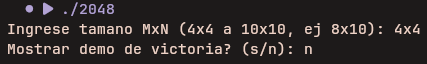
\includegraphics[width=0.85\textwidth]{imagenes/start-prompts.png}
	\caption{Entradas iniciales del juego.}
	\label{fig:start-prompts}
\end{figure}

\section{Controles}

Durante la partida se utilizan las flechas del teclado:

\begin{center}
\begin{tabular}{>{\raggedright\arraybackslash}p{0.35\textwidth} >{\raggedright\arraybackslash}p{0.45\textwidth}}
\toprule
\textbf{Tecla} & \textbf{Accion} \\
\midrule
Flecha izquierda & Desplazar fichas a la izquierda \\
Flecha derecha & Desplazar fichas a la derecha \\
Flecha arriba & Desplazar fichas hacia arriba \\
Flecha abajo & Desplazar fichas hacia abajo \\
\bottomrule
\end{tabular}
\end{center}

\section{Interfaz del juego}

La pantalla del juego contiene:
\begin{itemize}
	\item \textbf{Tablero}: muestra las fichas y sus valores.
	\item \textbf{Score}: puntaje acumulado por combinaciones.
	\item \textbf{Time}: tiempo transcurrido.
	\item \textbf{Mensajes de estado}: victoria o derrota.
\end{itemize}

\begin{figure}[H]
	\centering
	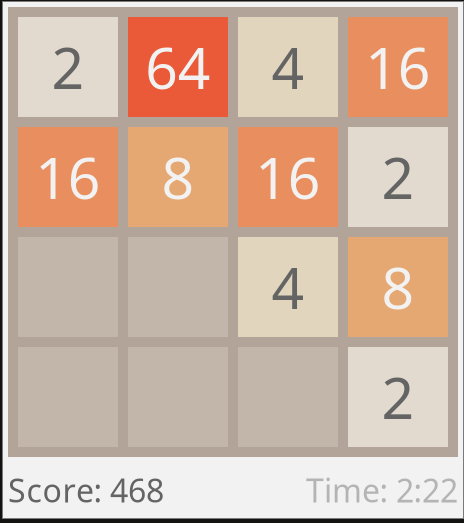
\includegraphics[width=0.5\textwidth]{imagenes/ui-main.png}
	\caption{Elementos de la interfaz.}
	\label{fig:ui-main}
\end{figure}

\section{Reglas de juego}

\begin{enumerate}
	\item Al mover en una direccion, todas las fichas intentan desplazarse en esa direccion.
	\item Si dos fichas adyacentes tienen el mismo valor, se combinan en una sola ficha con valor doble.
	\item Despues de un movimiento valido, aparece una nueva ficha. Usualmente es 2 y, ocasionalmente, 4.
	\item El juego termina cuando:
	\begin{itemize}
		\item No hay movimientos disponibles.
		\item Se alcanza la condicion de victoria (ficha 2048 en modo normal).
	\end{itemize}
\end{enumerate}

\section{Mensajes de estado}

El sistema puede mostrar los siguientes mensajes:
\begin{itemize}
	\item \texttt{Ganaste! :D}
	\item \texttt{Fin del juego :(}
\end{itemize}

\begin{figure}[H]
	\centering
	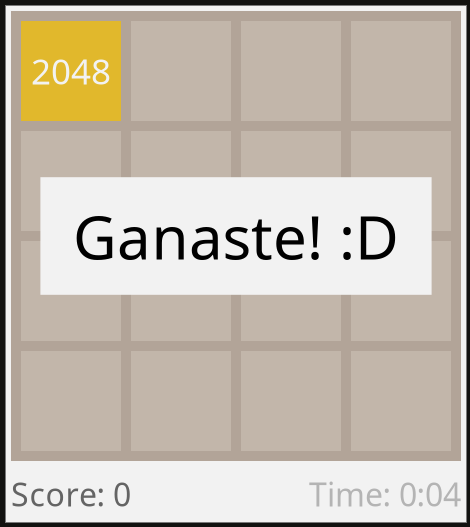
\includegraphics[width=0.5\textwidth]{imagenes/win-state.png}
	\caption{Mensaje de victoria.}
	\label{fig:win-state}
\end{figure}

\begin{figure}[H]
	\centering
	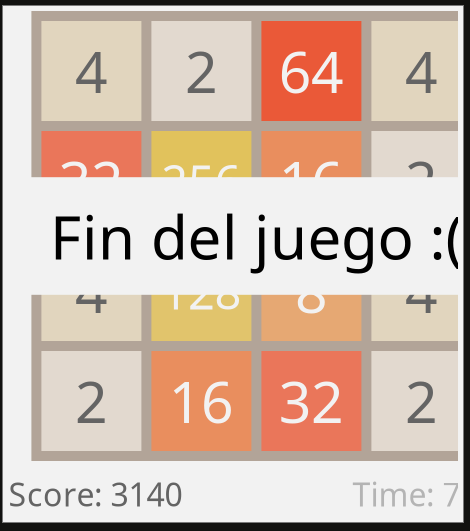
\includegraphics[width=0.5\textwidth]{imagenes/lose-state.png}
	\caption{Mensaje de fin de juego.}
	\label{fig:lose-state}
\end{figure}

\end{document}
